% - Privatisation of data
%   - Google, Facebook, NHS, Banks, retail stores (loyalty programs)
%   - Data Protection Act (limitations and corporate-focus)
% - User choice (who do I want to have my data and how)
% - Online identities
%   - Global identity tracking
%   - Conglomerate identity providers
\subsection{Motivation}

Over the last 350 years, the general public has, often unwittingly, handed their right to privacy over to corporations, conglomerates, and governments. This has occurred through the exchange of personal data for the convenience of the modern world. Some might argue, however, that these transactions have not occurred in good faith and have not been equally beneficial to both parties.
\newline
The origin of such transactions in the UK might be attributed to the introduction of paper money in 1694 by \cite{bankofengland:2016:online}. The introduction of paper currency gave an opportunity to the Bank of England to start collecting data on the exchange of money nationally. At the time it is unlikely that any person exchanging gold for paper currency was aware of the impending social shift, likely more concerned with the convenience afforded to them. Before this time, a person might have kept their savings 'under the mattress' and almost certainly would not have shared information relating to their wealth with another party. Whilst bank notes were introduced as a means to raise funds for war, the seed for a data revolution was inadvertently sewn. Whilst no unique identities were shared at this point, they would be in years to come.

Fast forward several hundred years and we find ourselves in a society where it is commonplace to rely on few key corporations and organisations to control information nationally and internationally. As (probably) the world's most popular social network~\footnote{\cite{worldmapsocialnetworks:2017:online}} it is clear from Facebook's terms and conditions~\footnote{\cite{facebookterms:2015:online}} that our use of the social network is subject to a few key conditions which restrict and change the status quo of our privacy as users. Foremost, it is apparent that whilst content posted on Facebook remains the property of the owner, Facebook has the right to use it how it wishes (as per the IP license) and hence is the controller of that data. One might choose to post their content on Facebook, but one cannot stop Facebook using their content without first removing it from all of Facebook's services and ensuring everyone with whom one has shared the content with has also removed it from Facebook. Furthermore this allows Facebook to use any content posted for machine learning, training systems, and providing commercial services using the intelligence gained from the distribution of content on the Facebook network. As someone who cares for their privacy, it is my opinion that this is not an acceptable status quo.

Notably, Facebook is not the only social network with this perspective on user privacy. Twitter also shares a very similar stance~\footnote{\cite{twittertos:2017:online}} and it is generally observed with most similar companies.

\begin{displayquote}{
  "\textbf{When it comes to control over our own data, health data must be where we draw the line.}"~\cite{wilbankstopol:2016:article}
}\end{displayquote}

% TODO: Swiss health identity card data

% - Privatisation of data
%   - Google, Facebook, NHS, Banks, retail stores (loyalty programs)
%   - Data Protection Act (limitations and corporate-focus)
% - User choice (who do I want to have my data and how)
% - Online identities
%   - Global identity tracking
%   - Conglomerate identity providers


At the core of the motivation for this project lay several issues corresponding to the way in which society has been manipulated over time. It is my belief that we find ourselves in the current position without any ownership of our data because we've been keen (even greedy) as a society to reap the benefits of our data without considering the longer term security effects. We have neglected our responsibility to care for our data.

Below, I have highlighted the key domains in which we lack control that we should have over our personal data. Whilst written as a piece of fiction, we should be aware and concerned that ignoring the social issues with data transfer allows a world to form much similar to that of George Orwell's 1984~\footnote{\cite{orwell:1984:book}} - we consider the likes of corporations synonymous with that of the 'Big Brother' character.

\subsubsection{Commoditisation of personal (and private) data}

There is no doubt that search tools such as those offered by Google and Microsoft, retail stores such as those offered by Amazon, and social networks such as Facebook and Twitter, dramatically enhance our lives and give us capabilities we would never have otherwise. Often as consumers we are eager to accept these benefits without considering the means by which they are offered to us. Every time we enter a search term into one of the websites above, or we buy something, or even when we click on a particular item in a store, a data point is generated. Whilst not valuable to us as consumers, that data point is the currency of choice of the multinationals. The more data points a corporation has per person, the easier it proves for them to accurately target you with information and offers that you will positively respond to.

For example, Amazon uses data gathered from it's own site and any other site where you interact with an Amazon-run entity (such as an advert)~\footnote{\href{https://www.amazon.com/b?node=5160028011}{Amazon Interest-based Ads}}. Whilst this exchange of data does mean you might receive offers more accustomed to your taste, it somewhat limits consumer choice and is designed such that the corporation makes the maximum profit.

\subsubsection{Retrieval of personal data}

As consumers we are not only exploited through data, but we also receive very little benefit from the data collected about us. Whilst we are able to share content using social networks and distribute this globally, other information is not so easily accessible.

As part of this project, I made a personal request to the NHS to get access to all data kept about myself. At first, the process seemed relatively simple and I hesitate to say that I was suprised. The NHS Digital response to my enquiry suggested that my health records may be available online and indeed this is suggested by the Patient Access service. Upon logging in however, I was greeted with screen in figure \ref{fig:patient_access_services}.

\begin{figure}[H]
  \centering
  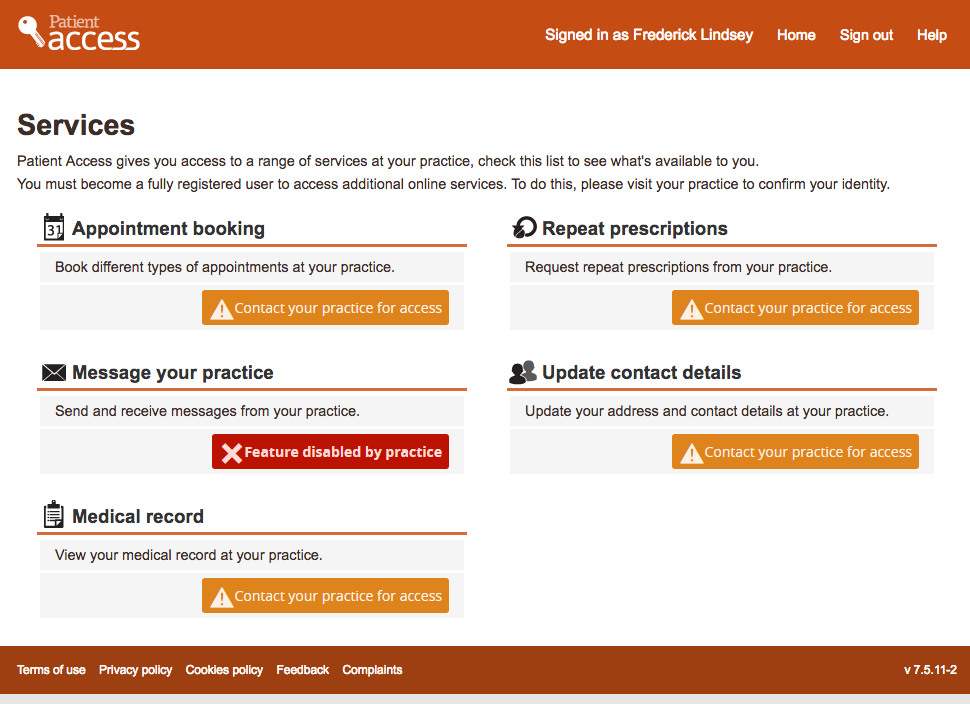
\includegraphics[width = 10cm]{images/patient_access_services.png} \\
  \caption{
  	Patient Access Services
  }{
    The services available to me (as of 13th June 2017) through Patient Access.
  }
  \label{fig:patient_access_services}
\end{figure}


The practice confirmed that whilst they recognise and are connected to the Patient Access service, they have no intention of connecting individual medical records they hold. Whilst it is possible to view your records informally with the supervision and guidance of a doctor, a formal request to receive a copy of the data held on file incurs financial implications\footnote{Data retrieval is at a cost of between £10 and £50 per item depending on its electronic/physical status. \href{https://www.gov.uk/government/publications/subject-access-request}{\textit{HSCIC Subject Request}}}

\subsubsection{Sharing of personal data, privately}

Central to the above two domains where we, as data providers, lose is the privacy and access to our data. It is necessary to question why we need to revoke all control over our data when we share it, why sharing data must exist in the public domain, and most importantly why we have somewhat limited right and ease to access any data generated about us.

Corporations (and their associated brands and trust) do provide some benefit in the sharing of data. If one were able to share a blob of data with another and prove that that data had been signed and created by an authority (a bank, doctor's surgery, hospital etc.) then the underlying data has increased value.

Once again considering patient records, we consider the treatment of a UK veteran with a disability (through ). The NHS states its commitment to veterans through offering priority treatment~\footnote{NHS offers priority treatment to all veterans based on clinical need. \href{http://www.nhs.uk/NHSEngland/Militaryhealthcare/veterans-families-reservists/Pages/veterans.aspx}{\textit{NHS Choices}}}. However, in order to be eligible a veteran must prove that their disability was caused by active service. Often requiring communication between the NHS and the armed forces, this is often a complicated and inefficient process. A solution to this problem whereby the patient would be able to share records (created by the armed forces) showing active service with the NHS and vice versa would be profound.
